\chapter{酶与生物化学催化}\label{ch:b1:enzymes}

将过氧化氢滴在切开的土豆上，它会起泡：土豆\omterm{def:b1:cell-unit-of-life:cell}{细胞}中的一个过氧化氢酶分子
每秒分解四千万个过氧化氢分子，
若任其自然，这一反应需要
数年时间。过氧化氢本身会分解——这一反应是放能的——
但在实用的时间内并不会发生。\omterm{def:b1:cell-unit-of-life:cell}{细胞}中的每一个反应都是如此：
热力学决定反应能朝哪个方向进行，
而\emph{酶}决定反应此刻是否发生。本章描述酶对反应的作用、
测定和比较酶所用的动力学、
酶受抑制的方式，以及\omterm{def:b1:cell-unit-of-life:cell}{细胞}
开启和关闭酶的方式。

\section{催化}

\begin{definition}[酶、底物与活性位点]\label{def:b1:enzymes:enzyme}
\emph{酶}\index{酶}是一类\omterm{def:b1:proteins:peptide}{蛋白质}（少数为 \omterm{def:b1:nucleic-acids:chain}{RNA}），它
能\emph{催化}一个反应：提高其速率，
自身不被消耗，也不改变平衡。被酶作用的分子称为
\emph{底物}\index{底物}，它们结合于
\emph{活性位点}\index{活性位点}，即由少数残基围成的裂隙，
反应的化学过程即在此处发生。酶是\emph{专一的}——作用于一种底物或一类底物，
作用于一个化学键或一种立体异构体——它们
依底物与反应类型命名，词尾为
\emph{-ase}（如乳糖酶、\omterm{def:b1:nucleic-acids:chain}{DNA} 聚合酶、琥珀酸脱氢酶），
并按反应类型分为六类：氧化还原酶、转移酶、水解酶、裂合酶、异构酶，
连接酶。许多酶需要非\omterm{def:b1:proteins:peptide}{蛋白质}的\emph{辅因子}\index{辅因子}：一个
金属离子（Zn、Mg、Fe），或一个有机的\emph{辅酶}\index{辅酶}
——$\mathrm{NAD^+}$、FAD、辅酶 A，它们大多由维生素合成而来，
这正是维生素的用途。
\end{definition}

\begin{proposition}[酶改变了什么，又未改变什么]\label{prop:b1:enzymes:whatitdoes}
\index{活化能}\index{过渡态}
反应经过一个\emph{\omterm{prop:b1:enzymes:whatitdoes}{过渡态}}，即原子的一种张紧构型，
其\omterm{prop:b1:water-small-molecules:gibbs}{自由能}比反应物或产物高出的量为
\emph{\omterm{prop:b1:enzymes:whatitdoes}{活化能}} $E_a$；只有
靠热运动越过这一能垒的分子才能反应，其比例
正比于 $e^{-E_a/RT}$。酶与\omterm{prop:b1:enzymes:whatitdoes}{过渡态}的结合
比与\omterm{def:b1:enzymes:enzyme}{底物}的结合更紧——其\omterm{def:b1:enzymes:enzyme}{活性位点}与张紧的构型互补，
从而使 $E_a$ 下降，
其降幅为 \qty{34}{kJ/mol}（相当于几个\omterm{def:b1:water-small-molecules:water}{氢键}的能量），在
\qty{37}{\celsius} 下，速率提高 $e^{34\,000/2580} \approx
10^6$ 倍。它不改变 $\Delta G$ 或平衡常数，
二者只取决于反应物与产物：酶使正向
与逆向反应的速率同等加快，使体系
更快地达到同一平衡。
\end{proposition}

\begin{omfigure}
\begin{tikzpicture}
\begin{axis}[
  width=0.86\linewidth, height=6.2cm,
  axis x line=bottom, axis y line=left,
  xmin=0, xmax=10, ymin=0, ymax=10,
  xlabel={反应坐标}, ylabel={自由能 $G$},
  xlabel style={font=\small, at={(axis description cs:0.5,-0.08)}, anchor=north},
  ylabel style={font=\small},
  xtick=\empty, ytick=\empty,
  clip=false,
]
\addplot[very thick, omDef, domain=0:10, samples=100, smooth] {5 + 4*exp(-((x-5)^2)/2.2) - 2.5/(1+exp(-(x-5)*1.5))};
\addplot[very thick, omThm, domain=0:10, samples=100, smooth] {5 + 1.6*exp(-((x-5)^2)/2.2) - 2.5/(1+exp(-(x-5)*1.5))};
\draw[<->, thick, omDef] (axis cs:5.6,5.0) -- (axis cs:5.6,8.95); \node[font=\scriptsize, omDef, anchor=west] at (axis cs:5.7,7.6) {无酶时 $E_a$};
\draw[<->, thick, omThm] (axis cs:4.4,5.0) -- (axis cs:4.4,6.55); \node[font=\scriptsize, omThm, anchor=east] at (axis cs:4.3,4.4) {有酶时 $E_a$};
\draw[<->, thick] (axis cs:9.3,2.5) -- (axis cs:9.3,5.0); \node[font=\scriptsize, anchor=west] at (axis cs:9.4,3.75) {$\Delta G$：不变};
\node[font=\scriptsize, anchor=north] at (axis cs:1.0,4.8) {底物};
\node[font=\scriptsize, anchor=north] at (axis cs:9.0,2.3) {产物};
\node[font=\scriptsize, anchor=south] at (axis cs:5,9.05) {过渡态};
\draw[dashed, gray] (axis cs:0,5) -- (axis cs:9.3,5);
\end{axis}
\end{tikzpicture}

{\small 沿反应进程的\omterm{prop:b1:water-small-molecules:gibbs}{自由能}。酶（红色）降低了
\omterm{prop:b1:enzymes:whatitdoes}{过渡态}的能垒，并使\omterm{def:b1:enzymes:enzyme}{底物}与产物之间的
能量差——进而平衡——保持不变。}
\end{omfigure}

\begin{omfigure}
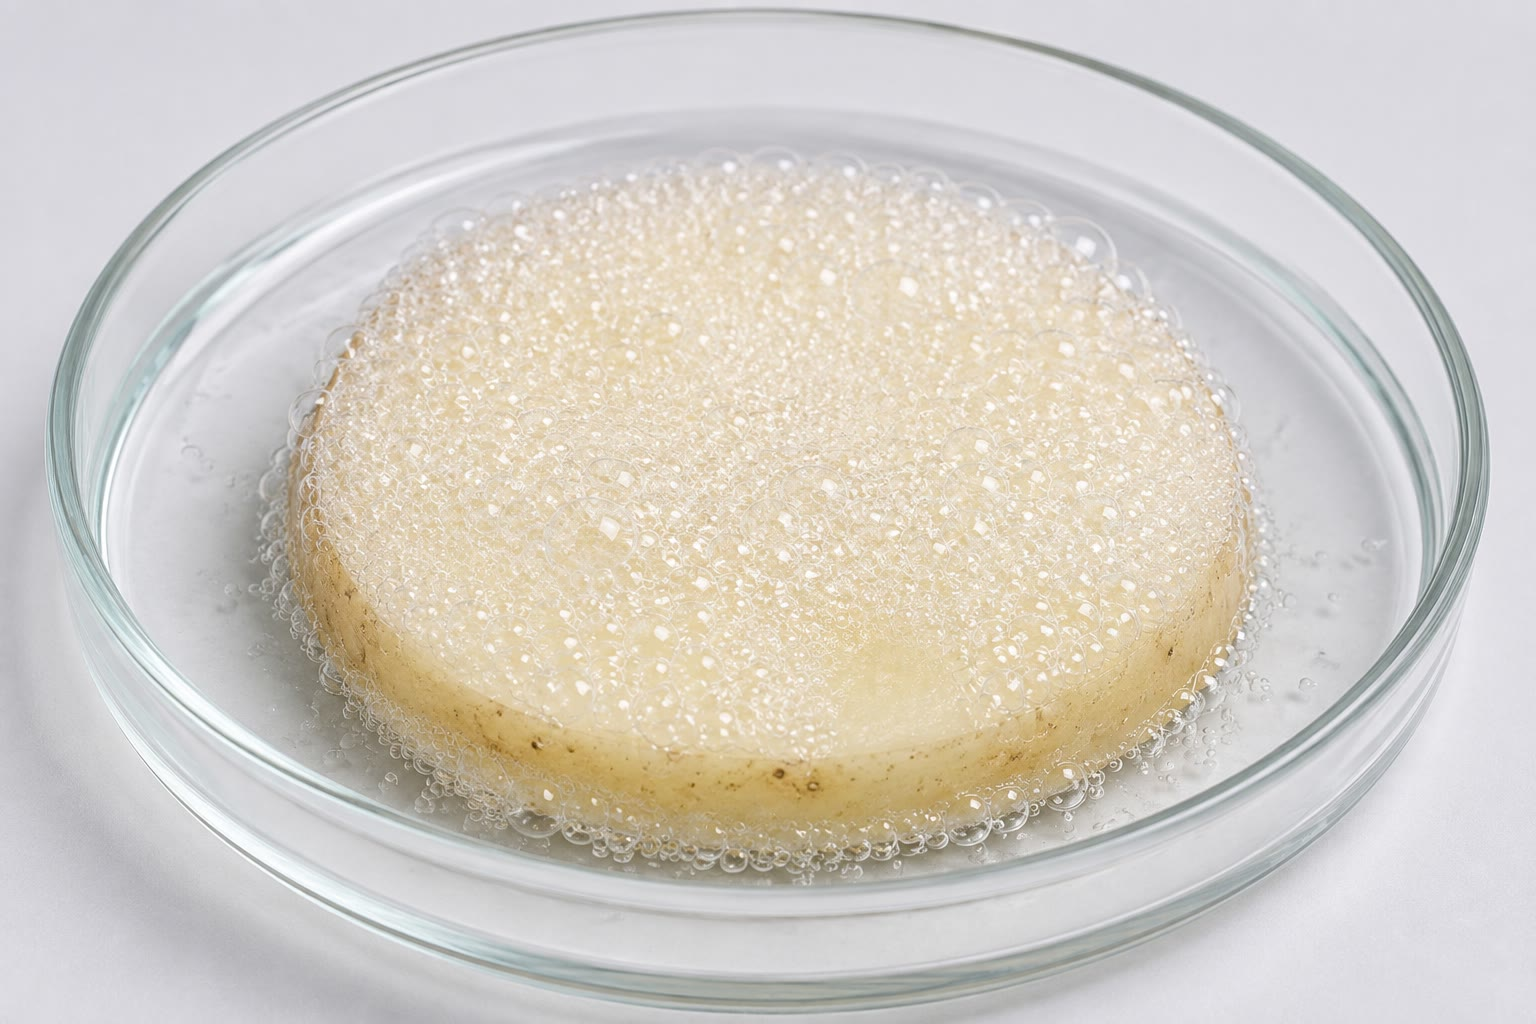
\includegraphics[width=0.5\linewidth]{images/book3/ai/b3-13-catalase-potato.jpg}

{\small 切开的土豆上的过氧化氢：\omterm{def:b1:cell-unit-of-life:cell}{细胞}中的过氧化氢酶
每秒钟，每个酶分子可将其分解为水和氧气四千万次，
氧气由此冒出气泡。}
\end{omfigure}

\begin{proposition}[活性位点的工作方式]\label{prop:b1:enzymes:mechanisms}
\omterm{def:b1:enzymes:enzyme}{活性位点}同时以多种方式加速其反应：它
\emph{结合并定向}\omterm{def:b1:enzymes:enzyme}{底物}，使反应基团
以正确的几何构型相遇，以确定的
碰撞取代罕见的偶然碰撞；它还使\omterm{def:b1:enzymes:enzyme}{底物}\emph{张紧}，趋向\omterm{prop:b1:enzymes:whatitdoes}{过渡态}
（\emph{诱导契合}\index{诱导契合}：酶包裹住
\omterm{def:b1:enzymes:enzyme}{底物}，且与\omterm{prop:b1:enzymes:whatitdoes}{过渡态}的契合最佳）；其\omterm{def:b1:proteins:aminoacid}{侧链}
起\emph{酸和碱}的作用，在适当时刻向\omterm{def:b1:enzymes:enzyme}{底物}
传递或接受质子（组氨酸的 p$K_a$ 接近 7，
在许多酶中如此）；有些酶会与\omterm{def:b1:enzymes:enzyme}{底物}形成短暂的\emph{\omterm{def:b1:water-small-molecules:bonds}{共价
键}}（如丝氨酸蛋白酶）；其金属离子
使键极化、稳定电荷。水大多被排斥在
\omterm{def:b1:enzymes:enzyme}{活性位点}之外，使电荷与\omterm{def:b1:water-small-molecules:water}{氢键}充分发挥作用。
\end{proposition}

\begin{example}[三种酶]\label{ex:b1:enzymes:three}
溶菌酶存在于泪液和蛋清中，它使细菌
\omterm{def:b1:eukaryotic-cell:plantcell}{细胞壁}中的一个糖环张紧成\omterm{prop:b1:enzymes:whatitdoes}{过渡态}的形状，并切断其链：
$10^8$ 倍加速。碳酸酐酶存在于红\omterm{def:b1:cell-unit-of-life:cell}{细胞}中，结合着
一个锌离子，它使水转化为氢氧根，随时准备进攻
$\mathrm{CO_2}$：每秒一百万个分子，是
仅次于过氧化氢酶的最快的酶。胰凝乳蛋白酶存在于胰液中，利用一个丝氨酸
经组氨酸活化，在芳香族残基之后切割\omterm{def:b1:proteins:peptide}{蛋白质}：
每秒一百次，并形成共价中间体。
\end{example}

\section{酶动力学}

\begin{definition}[初速率，饱和]\label{def:b1:enzymes:rate}
酶促反应的\emph{速率}\index{反应速率} $v$ 是
单位时间内生成的产物量（\unit{mol/s}，或以酶的
单位计：\qty{1}{\micro mol/min}）。它以\emph{初速率}测量，
即\omterm{def:b1:enzymes:enzyme}{底物}尚未耗尽、产物尚未积累之前的 $v_0$。
在酶浓度一定时，$v_0$ 随\omterm{def:b1:enzymes:enzyme}{底物}浓度
$[S]$ 升高，然后\emph{饱和}于
最大值 $V_{\max}$：此时酶已被完全占据，速率不能再升高。
\end{definition}

\begin{theorem}[米氏]\label{thm:b1:enzymes:mm}
\index{米氏方程}\index{米氏常数}
设酶 $E$ 可逆地结合其\omterm{def:b1:enzymes:enzyme}{底物}并将其转化，
\[
E + S \underset{k_{-1}}{\overset{k_1}{\rightleftharpoons}} ES
\overset{k_{\text{cat}}}{\longrightarrow} E + P ,
\]
\omterm{def:b1:enzymes:enzyme}{底物}浓度为 $[S]$ 时的初速率为
\[
v_0 = \frac{V_{\max}\,[S]}{K_m + [S]}, \qquad V_{\max} = k_{\text{cat}}\,[E]_{\text{tot}},
\qquad K_m = \frac{k_{-1} + k_{\text{cat}}}{k_1} .
\]
$K_m$，\emph{\omterm{thm:b1:enzymes:mm}{米氏常数}}，是
速率达到最大值一半时的\omterm{def:b1:enzymes:enzyme}{底物}浓度，它衡量酶需要多少\omterm{def:b1:enzymes:enzyme}{底物}；
$k_{\text{cat}}$，\emph{转化
数}\index{转化数}，指
饱和时一个酶分子每秒转化的\omterm{def:b1:enzymes:enzyme}{底物}分子数；比值
$k_{\text{cat}}/K_m$ 称为\emph{催化效率}，是
低\omterm{def:b1:enzymes:enzyme}{底物}浓度下的速率常数，其上限
由\omterm{def:b1:enzymes:enzyme}{底物}借扩散到达酶的速率决定，约为
$10^8$--$10^9$ \unit{L.mol^{-1}.s^{-1}}。
\end{theorem}
\begin{proof}
假设\emph{\omterm{def:b1:organism-environment:homeostasis}{稳态}}，即 $ES$ 的生成速率与其消失速率相等
（在最初几毫秒之后成立，此时 $[S] \gg [E]$）：
$k_1[E][S] = (k_{-1} + k_{\text{cat}})[ES]$，于是 $[E][S] = K_m[ES]$
其中 $K_m$ 如上定义。由守恒关系得 $[E] = [E]_{\text{tot}} -
[ES]$；代入得 $([E]_{\text{tot}} - [ES])[S] = K_m[ES]$，因此
$[ES] = [E]_{\text{tot}}[S]/(K_m + [S])$。速率为
$v_0 = k_{\text{cat}}[ES]$，由此得到上述公式；当 $[S] \gg K_m$ 时，
$v_0 \to k_{\text{cat}}[E]_{\text{tot}} = V_{\max}$，而在 $[S] = K_m$ 时，
$v_0 = V_{\max}/2$。
\end{proof}

\begin{omfigure}
\begin{minipage}[b]{0.52\linewidth}\centering
\begin{tikzpicture}
\begin{axis}[
  width=\linewidth, height=5.6cm,
  axis x line=bottom, axis y line=left,
  xmin=0, xmax=22, ymin=0, ymax=1.12,
  xlabel={$[S]$ (\unit{mmol/L})}, ylabel={$v_0$ (\unit{\micro mol/min})},
  xlabel style={font=\small, at={(axis description cs:0.5,-0.14)}, anchor=north},
  ylabel style={font=\small},
  tick label style={font=\small}, xtick={0,5,10,15,20}, ytick={0,0.5,1},
  clip=false,
]
\addplot[very thick, omDef, domain=0:22, samples=100] {x/(2+x)};
\addplot[only marks, mark=*, mark size=1.6pt, omDef!70!black] coordinates {(0.5,0.2) (1,0.333) (2,0.5) (5,0.714) (10,0.833) (20,0.909)};
\draw[dashed, gray] (axis cs:0,1) -- (axis cs:22,1); \node[font=\scriptsize, anchor=south east] at (axis cs:22,1.0) {$V_{\max}$};
\draw[dashed, gray] (axis cs:0,0.5) -- (axis cs:2,0.5) -- (axis cs:2,0); \node[font=\scriptsize, anchor=north] at (axis cs:2,-0.02) {$K_m$};
\end{axis}
\end{tikzpicture}
\end{minipage}\hfill
\begin{minipage}[b]{0.46\linewidth}\centering
\begin{tikzpicture}
\begin{axis}[
  width=\linewidth, height=5.6cm,
  axis x line=middle, axis y line=left,
  xmin=-0.7, xmax=2.2, ymin=0, ymax=5.5,
  xlabel={$1/[S]$}, ylabel={$1/v_0$},
  xlabel style={font=\small, at={(axis description cs:0.5,-0.14)}, anchor=north},
  ylabel style={font=\small},
  tick label style={font=\small}, xtick={0,1,2}, ytick={1,3,5},
  clip=false,
]
\addplot[very thick, omDef, domain=-0.5:2.1, samples=10] {1 + 2*x};
\addplot[only marks, mark=*, mark size=1.6pt, omDef!70!black] coordinates {(2,5) (1,3) (0.5,2) (0.2,1.4) (0.1,1.2) (0.05,1.1)};
\node[font=\scriptsize, anchor=west, align=left] at (axis cs:0.05,4.6) {斜率 $K_m/V_{\max}$};
\node[font=\scriptsize, anchor=west] at (axis cs:0.05,0.55) {$1/V_{\max}$};
\node[font=\scriptsize, anchor=south] at (axis cs:-0.5,0.1) {$-1/K_m$};
\end{axis}
\end{tikzpicture}
\end{minipage}

{\small 左图：米氏双曲线，对应 $K_m = \qty{2}{mmol/L}$
和 $V_{\max} = \qty{1}{\micro mol/min}$，并标出
周末问题中的六个测量点。右图：同一数据的莱恩威弗–伯克图，
即 $1/v_0$ 对 $1/[S]$ 作图：一条直线，其截距给出
$V_{\max}$ 和 $K_m$。}
\end{omfigure}

\begin{method}[测量 $K_m$ 与 $V_{\max}$]\label{met:b1:enzymes:lb}
\begin{enumerate}
  \item 配制一系列\omterm{def:b1:enzymes:enzyme}{底物}浓度，范围从
        $K_m/4$ 至 $10K_m$，酶浓度保持相同；跟踪
        产物（颜色、吸光度、气体）在第一分钟内的变化，并
        取其斜率作为 $v_0$。
  \item 作 $v_0$ 对 $[S]$ 的图：双曲线给出粗略的
        $V_{\max}$（平台值）和 $K_m$（对应
        平台值一半时的\omterm{def:b1:enzymes:enzyme}{底物}浓度）。
  \item 为求精确，取倒数：$1/v_0 = (K_m/V_{\max})(1/[S]) +
        1/V_{\max}$（\emph{莱恩威弗–伯克}）。该直线的截距
        在 $y$ 轴上为 $1/V_{\max}$，在 $x$ 轴上为 $-1/K_m$，其
        斜率为 $K_m/V_{\max}$。
  \item 将 $V_{\max}$ 除以酶浓度，得到
        $k_{\text{cat}}$；再除以 $K_m$ 得到效率。加入\omterm{def:b1:enzymes:inhibitors}{抑制剂}后重复
        实验，观察哪一参数发生变化。
\end{enumerate}
\end{method}

\begin{omfigure}
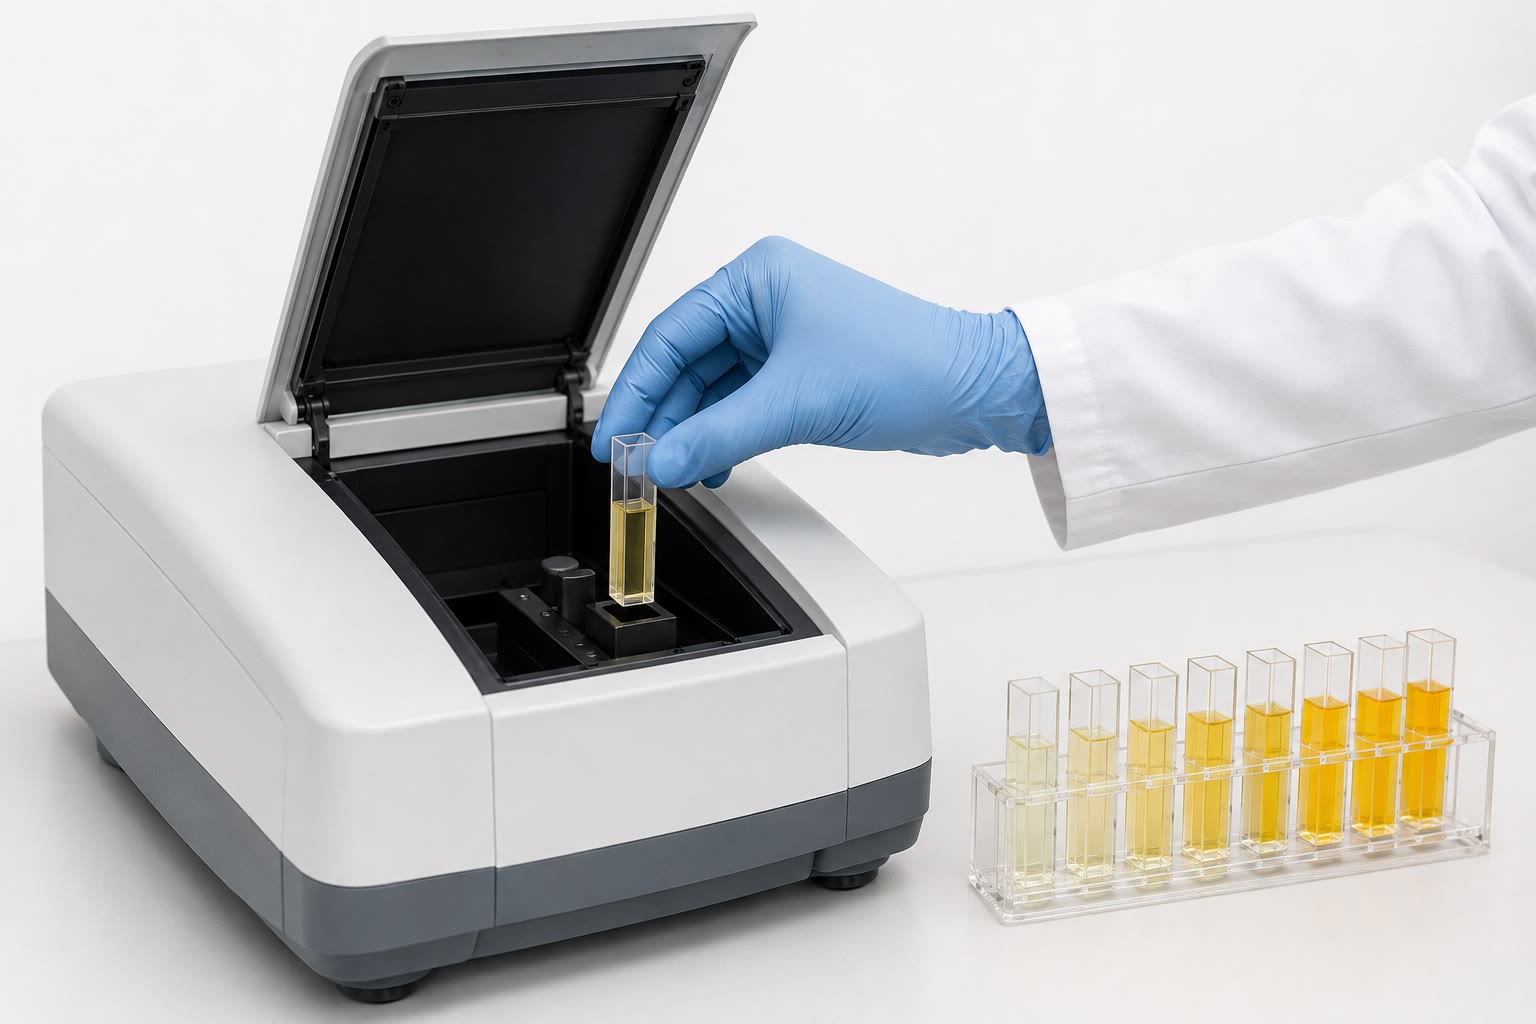
\includegraphics[width=0.5\linewidth]{images/book3/ai/b3-13-spectrophotometer-cuvette.jpg}

{\small 酶活性测定：产物吸收光，分光光度计
逐秒记录其吸光度的增长；初始斜率即
为 $v_0$。}
\end{omfigure}

\begin{example}[比较几种酶]\label{ex:b1:enzymes:compare}
\begin{center}
\small
\begin{tabular}{lccc}
\hline
酶 & $K_m$（\unit{mol/L}） & $k_{\text{cat}}$（\unit{s^{-1}}） & $k_{\text{cat}}/K_m$（\unit{L.mol^{-1}.s^{-1}}） \\
\hline
过氧化氢酶 & \num{2.5e-2} & \num{4e7} & \num{1.6e9} \\
碳酸酐酶 & \num{1.2e-2} & \num{1e6} & \num{8e7} \\
胰凝乳蛋白酶 & \num{1.5e-2} & 100 & \num{7e3} \\
溶菌酶 & \num{6e-6} & 0.5 & \num{8e4} \\
\omterm{def:b1:nucleic-acids:chain}{DNA} 聚合酶 & \num{1e-5} & 15 & \num{1.5e6} \\
\hline
\end{tabular}
\end{center}
过氧化氢酶和碳酸酐酶的催化已达扩散极限：每一次
与\omterm{def:b1:enzymes:enzyme}{底物}的碰撞都会生成产物。胰凝乳蛋白酶很慢，
但它必须如此——它切断的是\omterm{def:b1:proteins:peptide}{肽键}，比分解
过氧化物难得多。
\end{example}

\section{抑制作用}

\begin{definition}[抑制剂]\label{def:b1:enzymes:inhibitors}
\emph{抑制剂}\index{酶抑制剂}会降低
酶的反应速率。\emph{不可逆}抑制剂与酶共价结合，
永久性地破坏酶的活性（神经毒剂作用于乙酰胆碱酯酶，
青霉素作用于催化细菌\omterm{def:b1:eukaryotic-cell:plantcell}{细胞壁}交联的酶，阿司匹林作用于
合成前列腺素的酶）。\emph{可逆}抑制剂
通过弱键结合，可被洗脱；按结合位置分为：
\begin{itemize}
  \item \emph{竞争性}\index{竞争性抑制}：抑制剂
        与\omterm{def:b1:enzymes:enzyme}{底物}结构相似，占据\omterm{def:b1:enzymes:enzyme}{活性位点}；
        使表观 $K_m$ 升高（升高因子为 $1 + [I]/K_i$），
        而 $V_{\max}$ 不变——\omterm{def:b1:enzymes:enzyme}{底物}足够多时即可将其置换；
  \item \emph{非竞争性}：抑制剂结合于别处，
        无论是否结合\omterm{def:b1:enzymes:enzyme}{底物}，都会妨碍催化；它
        使 $V_{\max}$ 降低，而 $K_m$ 不变——再多的
        \omterm{def:b1:enzymes:enzyme}{底物}也无法克服它；
  \item \emph{反竞争性}：抑制剂只结合 $ES$
        复合物；$V_{\max}$ 和 $K_m$ 均降低。
\end{itemize}
$K_i$ 为抑制剂的解离常数，用以衡量其
效力：数值越小，抑制作用越强。
\end{definition}

\begin{omfigure}
\begin{tikzpicture}
\begin{axis}[
  width=0.8\linewidth, height=6.0cm,
  axis x line=middle, axis y line=left,
  xmin=-0.8, xmax=2.2, ymin=0, ymax=10.5,
  xlabel={$1/[S]$}, ylabel={$1/v_0$},
  xlabel style={font=\small, at={(axis description cs:0.5,-0.1)}, anchor=north},
  ylabel style={font=\small},
  tick label style={font=\small}, xtick={0,1,2}, ytick={2,4,6,8,10},
  legend style={font=\small, at={(0.03,0.97)}, anchor=north west, draw=none},
  clip=false,
]
\addplot[very thick, omDef, domain=-0.5:2.1, samples=10] {1 + 2*x};
\addlegendentry{无抑制剂}
\addplot[very thick, omThm, domain=-0.25:2.1, samples=10] {1 + 4*x};
\addlegendentry{竞争性：$1/V_{\max}$ 不变，斜率变大}
\addplot[very thick, omProp, domain=-0.5:2.1, samples=10] {2 + 4*x};
\addlegendentry{非竞争性：$-1/K_m$ 不变，纵截距升高}
\end{axis}
\end{tikzpicture}

{\small 两种常见\omterm{def:b1:enzymes:inhibitors}{抑制剂}的莱恩威弗–伯克图。
\omterm{def:b1:enzymes:inhibitors}{竞争性抑制}剂使直线绕 $y$ 轴截距转动
（$V_{\max}$ 不变，$K_m$ 升高）；非\omterm{def:b1:enzymes:inhibitors}{竞争性抑制}剂使其
绕 $x$ 轴截距转动（$K_m$ 不变，$V_{\max}$ 降低）。}
\end{omfigure}

\begin{example}[竞争作为药物]\label{ex:b1:enzymes:medicine}
甲醇本身无害，直到肝脏中的醇脱氢酶将其
转化为甲醛和甲酸，二者可致盲、致死。治疗
方法是使用乙醇：一种\omterm{def:b1:enzymes:inhibitors}{竞争性}\omterm{def:b1:enzymes:enzyme}{底物}，其 $K_m$ 更低，能使
酶保持忙碌，甲醇则原样排出。他汀类药物是
\omterm{def:b1:enzymes:inhibitors}{竞争性抑制}剂，结构类似\omterm{prop:b1:enzymes:whatitdoes}{过渡态}，作用于
使碳转向\omterm{def:b1:lipids:amphiphilic}{胆固醇}的酶；磺胺类药物的结构类似
细菌合成叶酸的酶的\omterm{def:b1:enzymes:enzyme}{底物}，人体不能合成叶酸，
因而不受影响。
\end{example}

\section{调节}

\begin{definition}[别构酶]\label{def:b1:enzymes:allosteric}
\emph{别构酶}\index{别构酶}含有多个亚基，
除\omterm{def:b1:enzymes:enzyme}{活性位点}外，还有\emph{调节位点}，效应物
在其上结合：\emph{激活剂}使其趋向活性
\emph{\omterm{def:b1:enzymes:inhibitors}{抑制剂}}使其趋向非活性构象。其反应速率
随 $[S]$ 的变化呈 S 形，而非双曲线形（\omterm{def:b1:enzymes:enzyme}{活性位点}之间存在协同作用
，如血红蛋白，见\cref{ch:b1:proteins}），因此
\omterm{def:b1:enzymes:enzyme}{底物}浓度在陡峭段附近的微小变化会使速率
大幅改变；效应物既可使曲线横向平移（改变
所需的\omterm{def:b1:enzymes:enzyme}{底物}浓度），也可使曲线上下移动（改变最大速率）。
别构酶位于代谢的分支点，而
效应物即代谢途径自身的产物和\omterm{def:b1:cell-unit-of-life:cell}{细胞}的能量
信号（\omterm{def:b1:water-small-molecules:atp}{ATP}、ADP、AMP）。
\end{definition}

\begin{omfigure}
\begin{tikzpicture}
\begin{axis}[
  width=0.86\linewidth, height=6.0cm,
  axis x line=bottom, axis y line=left,
  xmin=0, xmax=10, ymin=0, ymax=1.1,
  xlabel={$[S]$（相对值）}, ylabel={$v_0/V_{\max}$},
  xlabel style={font=\small, at={(axis description cs:0.5,-0.12)}, anchor=north},
  ylabel style={font=\small},
  tick label style={font=\small}, xtick={0,2,4,6,8,10}, ytick={0,0.5,1},
  legend style={font=\small, at={(0.5,-0.22)}, anchor=north, draw=none, legend columns=2, /tikz/every even column/.append style={column sep=0.4cm}},
  clip=false,
]
\addplot[very thick, omDef, domain=0:10, samples=100] {x^3/(3^3+x^3)};
\addlegendentry{单独的别构酶（$n = 3$）}
\addplot[very thick, omExo, domain=0:10, samples=100] {x^3/(1.8^3+x^3)};
\addlegendentry{加激活剂：曲线左移}
\addplot[very thick, omThm, domain=0:10, samples=100] {x^3/(5.5^3+x^3)};
\addlegendentry{加抑制剂：曲线右移}
\addplot[thick, dashed, gray, domain=0:10, samples=100] {x/(3+x)};
\addlegendentry{米氏方程，作比较}
\draw[dashed, gray] (axis cs:3,0) -- (axis cs:3,0.5);
\end{axis}
\end{tikzpicture}

{\small 一种\omterm{def:b1:enzymes:allosteric}{别构酶}。S 形曲线使速率在中点附近对\omterm{def:b1:enzymes:enzyme}{底物}十分敏感；
激活剂使其左移（在给定的 $[S]$ 下活性更高），
\omterm{def:b1:enzymes:inhibitors}{抑制剂}使其右移。在 $[S] = 3$ 附近，
速率可从最大值的十分之一变化到十分之九。}
\end{omfigure}

\begin{proposition}[细胞控制酶的四种方式]\label{prop:b1:enzymes:control}
\begin{enumerate}
  \item \emph{反馈抑制}\index{反馈抑制}：途径的终产物
        是其首个承诺性酶的别构\omterm{def:b1:enzymes:inhibitors}{抑制剂}，使途径只以终产物被利用的速度运行
        （异亮氨酸作用于苏氨酸脱氨酶；
        \omterm{def:b1:water-small-molecules:atp}{ATP} 作用于
        磷酸果糖激酶（见\cref{ch:b1:respiration-fermentation}）。
        响应时间：毫秒级。
  \item \emph{共价修饰}\index{共价修饰}：激酶将磷酸基团
        连接到酶的丝氨酸、苏氨酸或酪氨酸上，磷酸酶则将其去除，
        两种形式的活性不同（\omterm{def:b1:carbohydrates:polysaccharide}{糖原}磷酸化酶在同一
        激素信号下通过磷酸化被激活，\omterm{def:b1:carbohydrates:polysaccharide}{糖原}合酶则被关闭）。
        响应时间为秒至分钟级，
        可逆，
        可在级联中\omterm{def:b1:cell-unit-of-life:resolution}{放大}。
  \item \emph{蛋白水解激活}：有些酶以无活性的前体形式合成
        （\emph{酶原}：胰蛋白酶原、胃蛋白酶原、凝血因子），
        通过切去一段肽段而被激活，
        这是一次性的不可逆过程，
        在需要之处、需要之时发生。
  \item \emph{数量}：\omterm{def:b1:cell-unit-of-life:cell}{细胞}通过调控自身基因
        （见\cref{ch:b1:expression-control}）来增减酶的合成量，并以或快或慢的速度降解它。
        响应时间为分钟至小时级。
\end{enumerate}
\end{proposition}

\begin{example}[同工酶]\label{ex:b1:enzymes:isoenzymes}
乳酸脱氢酶有五种形式，由两类亚基以各种组合构成的四聚体；
心脏的形式对乳酸的 $K_m$ 较低，
并受丙酮酸抑制（它将乳酸氧化，为
克雷布斯循环提供\omterm{def:b1:enzymes:enzyme}{底物}），肌肉的形式 $V_{\max}$ 较高，且能耐受丙酮酸
（它在短跑时生成乳酸）。血液中各种形式的分布
可以揭示哪个\omterm{def:b1:mammal-organization:organ}{器官}受损：心脏病发作时释放出的是
心脏的形式。
\end{example}

\section{温度与 pH}

\begin{proposition}[酶及其环境]\label{prop:b1:enzymes:environment}
酶促反应速率每升高
\qty{10}{\celsius}（$Q_{10} \approx 2$），大致翻一倍，因为热能使更多
分子越过能垒，直到酶开始\omterm{def:b1:nucleic-acids:melting}{变性}
（大多数酶为 \qtyrange{40}{60}{\celsius}；温泉细菌的酶为
\qty{100}{\celsius}），反应速率随之急剧下降。每种酶都有
一个\emph{最适 \omterm{def:b1:water-small-molecules:ph}{pH}}，在此 \omterm{def:b1:water-small-molecules:ph}{pH} 下其催化残基和\omterm{def:b1:enzymes:enzyme}{底物}的解离状态恰当：
胃蛋白酶在胃中，最适 \omterm{def:b1:water-small-molecules:ph}{pH} 约为 2；胰蛋白酶在肠中，约为 8；
大多数\omterm{def:b1:cell-unit-of-life:cell}{细胞}内酶约为 7。
偏离最适值时速率下降，偏离很远时\omterm{def:b1:proteins:peptide}{蛋白质}\omterm{def:b1:nucleic-acids:melting}{变性}。
温度和 \omterm{def:b1:water-small-molecules:ph}{pH} 都作用于\omterm{def:b1:proteins:peptide}{蛋白质}；\omterm{def:b1:cell-unit-of-life:cell}{细胞}将二者维持在
其上千种酶都能正常工作的范围内。
\end{proposition}

\begin{example}[发热与温泉]\label{ex:b1:enzymes:fever}
发热至 \qty{40}{\celsius} 时，体内每个反应的速度加快约四分之一，
并开始使最脆弱的\omterm{def:b1:proteins:peptide}{蛋白质}\omterm{def:b1:nucleic-acids:melting}{变性}；在
\qty{42}{\celsius} 时大脑功能便会失效。一种细菌的 \omterm{def:b1:nucleic-acids:chain}{DNA} 聚合酶，
取自 \qty{75}{\celsius} 温泉，能耐受 \qty{95}{\celsius}，因此
可以反复经历数千次 \omterm{def:b1:nucleic-acids:chain}{DNA} 熔化而循环使用，
并成为聚合酶链式反应（本科三年级分册）的酶。
耐热性是序列的性质，
而不是所催化反应的性质。
\end{example}

\section{练习}

\begin{exercise}[$\star$]\label{exo:b1:enzymes:1}
酶在反应中改变了什么，又保持了什么不变？
请借助能量曲线加以说明。
\end{exercise}

\begin{exercise}[$\star$]\label{exo:b1:enzymes:2}
定义 $K_m$、$V_{\max}$、$k_{\text{cat}}$ 和 $k_{\text{cat}}/K_m$，
并注明单位。
\end{exercise}

\begin{exercise}[$\star$]\label{exo:b1:enzymes:3}
由\omterm{def:b1:enzymes:inhibitors}{抑制剂}的莱恩威弗–伯克图，读出 $V_{\max}$
以及 $K_m$，分别针对未受抑制的酶和各\omterm{def:b1:enzymes:inhibitors}{抑制剂}。
\end{exercise}

\begin{exercise}[$\star$]\label{exo:b1:enzymes:4}
说出\omterm{def:b1:cell-unit-of-life:cell}{细胞}调节酶活性的四种方式，
并给出每种方式的时间尺度。
\end{exercise}

\begin{exercise}[$\star\star$]\label{exo:b1:enzymes:5}
某酶的 $K_m = \qty{0.1}{mmol/L}$，$V_{\max} =
\qty{50}{\micro mol/min}$。计算 $v_0$，取 $[S] = 0.02$、$0.1$、$1$
和 \qty{10}{mmol/L} 时的值。$[S]$ 为何值时 $v_0 = 0.9\,V_{\max}$？
\end{exercise}

\begin{exercise}[$\star\star$]\label{exo:b1:enzymes:6}
在 \qty{37}{\celsius} 下将 $E_a$ 降低 \qty{20}{kJ/mol}，
速率变为原来的多少倍？$E_a$ 需降低多少，
才能使速率增大 $10^{10}$ 倍？
\end{exercise}

\begin{exercise}[$\star\star$]\label{exo:b1:enzymes:7}
$\qty{2}{pmol}$ 碳酸酐酶溶于 \qty{1}{mL} 中，
测得 $V_{\max} = \qty{120}{mmol/L}$（每分钟）。计算 $k_{\text{cat}}$，
并在 $K_m = \qty{12}{mmol/L}$ 时求效率，
再与扩散极限比较。
\end{exercise}

\begin{exercise}[$\star\star$]\label{exo:b1:enzymes:8}
\omterm{def:b1:enzymes:inhibitors}{竞争性抑制}剂在 \qty{2}{mmol/L} 时使表观 $K_m$ 加倍。
计算 $K_i$。有与无\omterm{def:b1:enzymes:inhibitors}{抑制剂}时，各需多大\omterm{def:b1:enzymes:enzyme}{底物}浓度，
才能使速率恢复到 $V_{\max}$ 的 \qty{90}{\%}，
若 $K_m = \qty{1}{mmol/L}$？
\end{exercise}

\begin{exercise}[$\star\star$]\label{exo:b1:enzymes:9}
解释为何\omterm{prop:b1:enzymes:control}{反馈抑制}作用于途径中的第一个承诺步骤，
而非最后一步，并说明为何\omterm{def:b1:enzymes:inhibitors}{抑制剂}通常是
终产物而非中间产物。
\end{exercise}

\begin{exercise}[$\star\star\star$]\label{exo:b1:enzymes:10}
胰蛋白酶原在肠道中被激活，而非在合成它的胰腺中被激活；
少量过早激活便会破坏胰腺。
解释酶原的作用逻辑、激活胰蛋白酶原的酶的作用，
以及胰腺为何同时合成胰蛋白\omterm{def:b1:enzymes:inhibitors}{酶抑制剂}。
\end{exercise}

\begin{exercise}[$\star\star\star$]\label{exo:b1:enzymes:11}
一种\omterm{def:b1:enzymes:allosteric}{别构酶}，$n = 3$，半饱和浓度 $[S]_{0.5}
= 3$，加入\omterm{def:b1:enzymes:inhibitors}{抑制剂}后其曲线移至 $[S]_{0.5} = 5.5$。
计算 $[S] = 3$ 时有、无\omterm{def:b1:enzymes:inhibitors}{抑制剂}的速率，并
与同样使 $K_m$ 移动相同幅度的\omterm{def:b1:enzymes:inhibitors}{竞争性抑制}剂
作用于米氏酶时所产生的变化相比较。
\omterm{def:b1:proteins:allostery}{协同性}为调节增添了什么？
\end{exercise}

\begin{exercise}[$\star\star\star$]\label{exo:b1:enzymes:12}
“酶是一种被告知该做什么的催化剂。”用一段文字讨论：
催化与专一性；作为附加信息的调节；
以及受调节的酶相对于裸露的
催化剂所付出的代价。
\end{exercise}

\section{问题：测定一种酶}

\begin{problem}[{周末问题——测定一种酯酶在六种\omterm{def:b1:enzymes:enzyme}{底物}浓度下的活性，
分别在单独存在及有两种\omterm{def:b1:enzymes:inhibitors}{抑制剂}时进行，提取其常数，
并预测其在\omterm{def:b1:cell-unit-of-life:cell}{细胞}中的行为，最终求出其 $K_m$、
$V_{\max}$ 和 $K_i$}]
\label{pb:b1:enzymes:1}
在 \qty{1.0}{mL} 体系中、\qty{25}{\celsius}、\omterm{def:b1:water-small-molecules:ph}{pH} 7.5 条件下测定一种酯酶，
酶的浓度为 \qty{10}{nmol/L}。初速率（单位 \unit{\micro mol/min}）见下，
为六种\omterm{def:b1:enzymes:enzyme}{底物}浓度下的值，分别在单独存在时，以及存在
\qty{1.0}{mmol/L} \omterm{def:b1:enzymes:inhibitors}{抑制剂} I 或 \qty{1.0}{mmol/L} \omterm{def:b1:enzymes:inhibitors}{抑制剂} J 时测得：

\begin{center}
\small
\begin{tabular}{lcccccc}
\hline
$[S]$ (\unit{mmol/L}) & 0.5 & 1 & 2 & 5 & 10 & 20 \\
\hline
$v_0$，无\omterm{def:b1:enzymes:inhibitors}{抑制剂} & 0.200 & 0.333 & 0.500 & 0.714 & 0.833 & 0.909 \\
$v_0$，含 I & 0.111 & 0.200 & 0.333 & 0.556 & 0.714 & 0.833 \\
$v_0$，含 J & 0.100 & 0.167 & 0.250 & 0.357 & 0.417 & 0.455 \\
\hline
\end{tabular}
\end{center}

\medskip
\noindent\textbf{第一部分——单独的酶。}
\begin{enumerate}
  \item 对无\omterm{def:b1:enzymes:inhibitors}{抑制剂}的六个数据点，
        计算 $1/[S]$ 和 $1/v_0$。
  \item 证明这些点位于同一直线上，并求出其
        斜率与截距。
  \item 由此推出 $V_{\max}$ 与 $K_m$。
  \item 用\omterm{thm:b1:enzymes:mm}{米氏方程}，在 $[S] =
        \qty{5}{mmol/L}$ 处进行验证。
  \item 计算测定体系中酶的量（以摩尔计）以及
        $k_{\text{cat}}$（单位 \unit{s^{-1}}）。
  \item 计算 $k_{\text{cat}}/K_m$，并与扩散极限
        比较。
  \item 酶在何种\omterm{def:b1:enzymes:enzyme}{底物}浓度下以
        \qty{95}{\%} 的 $V_{\max}$ 工作？
\end{enumerate}

\medskip
\noindent\textbf{第二部分——\omterm{def:b1:enzymes:inhibitors}{抑制剂} I。}
\begin{enumerate}[resume]
  \item 对含 I 的六个数据点，计算 $1/v_0$，并求出其
        直线的斜率与截距。
  \item 由此推出含 I 时的表观 $V_{\max}$ 与 $K_m$。
  \item 哪一参数发生了变化？对该\omterm{def:b1:enzymes:inhibitors}{抑制剂}进行分类。
  \item 计算 $K_i$，依据 $K_m^{\text{app}} = K_m(1 + [I]/K_i)$。
  \item 在 $[S] = \qty{2}{mmol/L}$ 时，多大浓度的 I 能使
        速率减半？在 $[S] = \qty{20}{mmol/L}$ 时又如何？
  \item 从结构上推测 I 可能是什么，以及它结合在何处。
\end{enumerate}

\medskip
\noindent\textbf{第三部分——\omterm{def:b1:enzymes:inhibitors}{抑制剂} J。}
\begin{enumerate}[resume]
  \item 计算含 J 时直线的斜率与截距，
        由此推出表观 $V_{\max}$ 与 $K_m$。
  \item 对 J 分类，并计算其 $K_i$，依据 $V_{\max}^{\text{app}} =
        V_{\max}/(1 + [J]/K_i)$。
  \item 解释为何提高\omterm{def:b1:enzymes:enzyme}{底物}浓度无法克服 J 的抑制。
  \item 在存在 J 时将酶浓度加倍，速率
        如何变化？在存在 I 时又如何？
\end{enumerate}

\medskip
\noindent\textbf{第四部分——\omterm{def:b1:cell-unit-of-life:cell}{细胞}中的情况。}
\omterm{def:b1:cell-unit-of-life:cell}{细胞}内\omterm{def:b1:enzymes:enzyme}{底物}浓度为 \qty{0.5}{mmol/L}，酶浓度为
\qty{10}{nmol/L}，体积为 \qty{1000}{\micro m^3}，温度为
\qty{37}{\celsius}，$Q_{10} = 2$。
\begin{enumerate}[resume]
  \item 计算\omterm{def:b1:cell-unit-of-life:cell}{细胞}内的速率（整个\omterm{def:b1:cell-unit-of-life:cell}{细胞}中每秒产生的
        产物分子数）。
  \item \omterm{def:b1:cell-unit-of-life:cell}{细胞}需要以每秒 \qty{3e6}{} 个分子的速率获得该产物。
        \omterm{def:b1:cell-unit-of-life:cell}{细胞}须将速率提高到原来的多少倍，
        并说出两种可行的方式。
  \item 该产物为该酶的\omterm{def:b1:enzymes:inhibitors}{竞争性抑制}剂，其
        $K_i = \qty{0.2}{mmol/L}$，并积累至
        \qty{0.4}{mmol/L}，计算此时的速率，并
        说明这样做达到了什么效果。
  \item 该酶被一种激酶磷酸化，使其
        $K_m$ 降至 \qty{0.4}{mmol/L}。计算\omterm{def:b1:enzymes:enzyme}{底物}浓度为
        \qty{0.5}{mmol/L} 时修饰前后的速率。
  \item 该酶的最适 \omterm{def:b1:water-small-molecules:ph}{pH} 为 7.5，在 \omterm{def:b1:water-small-molecules:ph}{pH}
        6.5 时活性减半。\omterm{def:b1:eukaryotic-cell:endomembrane}{溶酶体}的 \omterm{def:b1:water-small-molecules:ph}{pH} 为 5，定性预测
        该酶在其中的活性，并依据可解离残基加以解释。
  \item 一次突变将\omterm{def:b1:enzymes:enzyme}{活性位点}的组氨酸替换为
        丙氨酸。预测其对 $K_m$ 与 $k_{\text{cat}}$ 的影响，
        并分别说明理由。
  \item 解释\omterm{def:b1:cell-unit-of-life:cell}{细胞}为何将\omterm{def:b1:enzymes:enzyme}{底物}浓度维持在 $K_m$ 附近，
        而不是远高于该值。
  \item 给出结果：酯酶的 $K_m$、$V_{\max}$、$k_{\text{cat}}$，
        以及各\omterm{def:b1:enzymes:inhibitors}{抑制剂}的类型与 $K_i$。
\end{enumerate}
\end{problem}
